% Options for packages loaded elsewhere
\PassOptionsToPackage{unicode}{hyperref}
\PassOptionsToPackage{hyphens}{url}
\documentclass[
]{article}
\usepackage{xcolor}
\usepackage[margin=1in]{geometry}
\usepackage{amsmath,amssymb}
\setcounter{secnumdepth}{-\maxdimen} % remove section numbering
\usepackage{iftex}
\ifPDFTeX
  \usepackage[T1]{fontenc}
  \usepackage[utf8]{inputenc}
  \usepackage{textcomp} % provide euro and other symbols
\else % if luatex or xetex
  \usepackage{unicode-math} % this also loads fontspec
  \defaultfontfeatures{Scale=MatchLowercase}
  \defaultfontfeatures[\rmfamily]{Ligatures=TeX,Scale=1}
\fi
\usepackage{lmodern}
\ifPDFTeX\else
  % xetex/luatex font selection
\fi
% Use upquote if available, for straight quotes in verbatim environments
\IfFileExists{upquote.sty}{\usepackage{upquote}}{}
\IfFileExists{microtype.sty}{% use microtype if available
  \usepackage[]{microtype}
  \UseMicrotypeSet[protrusion]{basicmath} % disable protrusion for tt fonts
}{}
\makeatletter
\@ifundefined{KOMAClassName}{% if non-KOMA class
  \IfFileExists{parskip.sty}{%
    \usepackage{parskip}
  }{% else
    \setlength{\parindent}{0pt}
    \setlength{\parskip}{6pt plus 2pt minus 1pt}}
}{% if KOMA class
  \KOMAoptions{parskip=half}}
\makeatother
\usepackage{graphicx}
\makeatletter
\newsavebox\pandoc@box
\newcommand*\pandocbounded[1]{% scales image to fit in text height/width
  \sbox\pandoc@box{#1}%
  \Gscale@div\@tempa{\textheight}{\dimexpr\ht\pandoc@box+\dp\pandoc@box\relax}%
  \Gscale@div\@tempb{\linewidth}{\wd\pandoc@box}%
  \ifdim\@tempb\p@<\@tempa\p@\let\@tempa\@tempb\fi% select the smaller of both
  \ifdim\@tempa\p@<\p@\scalebox{\@tempa}{\usebox\pandoc@box}%
  \else\usebox{\pandoc@box}%
  \fi%
}
% Set default figure placement to htbp
\def\fps@figure{htbp}
\makeatother
\setlength{\emergencystretch}{3em} % prevent overfull lines
\providecommand{\tightlist}{%
  \setlength{\itemsep}{0pt}\setlength{\parskip}{0pt}}
\usepackage{bookmark}
\IfFileExists{xurl.sty}{\usepackage{xurl}}{} % add URL line breaks if available
\urlstyle{same}
\hypersetup{
  pdftitle={Tutorial},
  hidelinks,
  pdfcreator={LaTeX via pandoc}}

\title{Tutorial}
\author{}
\date{\vspace{-2.5em}}

\begin{document}
\maketitle

\textbf{Choosing Analysis Tab \& General Considerations} The first thing
to understand before using this application is which analysis tab you
want to use. This depends on the type of variables you wish to form into
a composite and also the number of intervention groups.

The ``Analysis-SC/QC Composite'' tab is only suitable for composites
formed from binary and continuous variables, and for comparing only two
intervention groups. The ``Analysis-QC Composite'' tab can also handle
categorical data and survival analysis, as well as being able to compare
multiple intervention groups.

Note that only raw data and permutation testing can be used for the
``Analysis-QC Composite'' tab.

\textbf{Notes on raw data} Additionally, there are a few important
details which are required when uploading data. Raw data should be
uploaded as a csv file, in wide format, with all variables in numeric
format (excluding column names, if applicable). \textbf{Importantly} the
first column of the file should indicate an ID for each individual, and
the second column should indicate the intervention group. The following
columns should only include the relevant outcomes for creating the
composite (as all the following columns will be used to create the
composite test statistic). Also, ensure that there are no missing values
for treatment group. The data can also be uploaded with or without
column names, although we would recommend including column names for the
sake of simplicity. If column names are present, ensure that the
``Header'' check box is ticked as seen below. If your file does not
contain column names, ensure this check box is un-ticked.

\begin{center}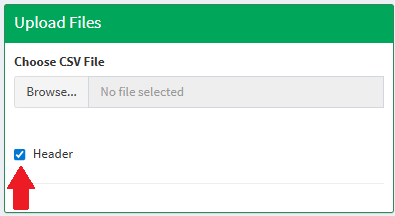
\includegraphics[width=5.49in]{Upload Files} \end{center}

Equal weighting is applied by default (w = 1). Once a valid raw data csv
file has been uploaded, input boxes for weights will appear for each
outcome, which can then be adjusted if necessary. See below an example
of how this might appear.

\begin{center}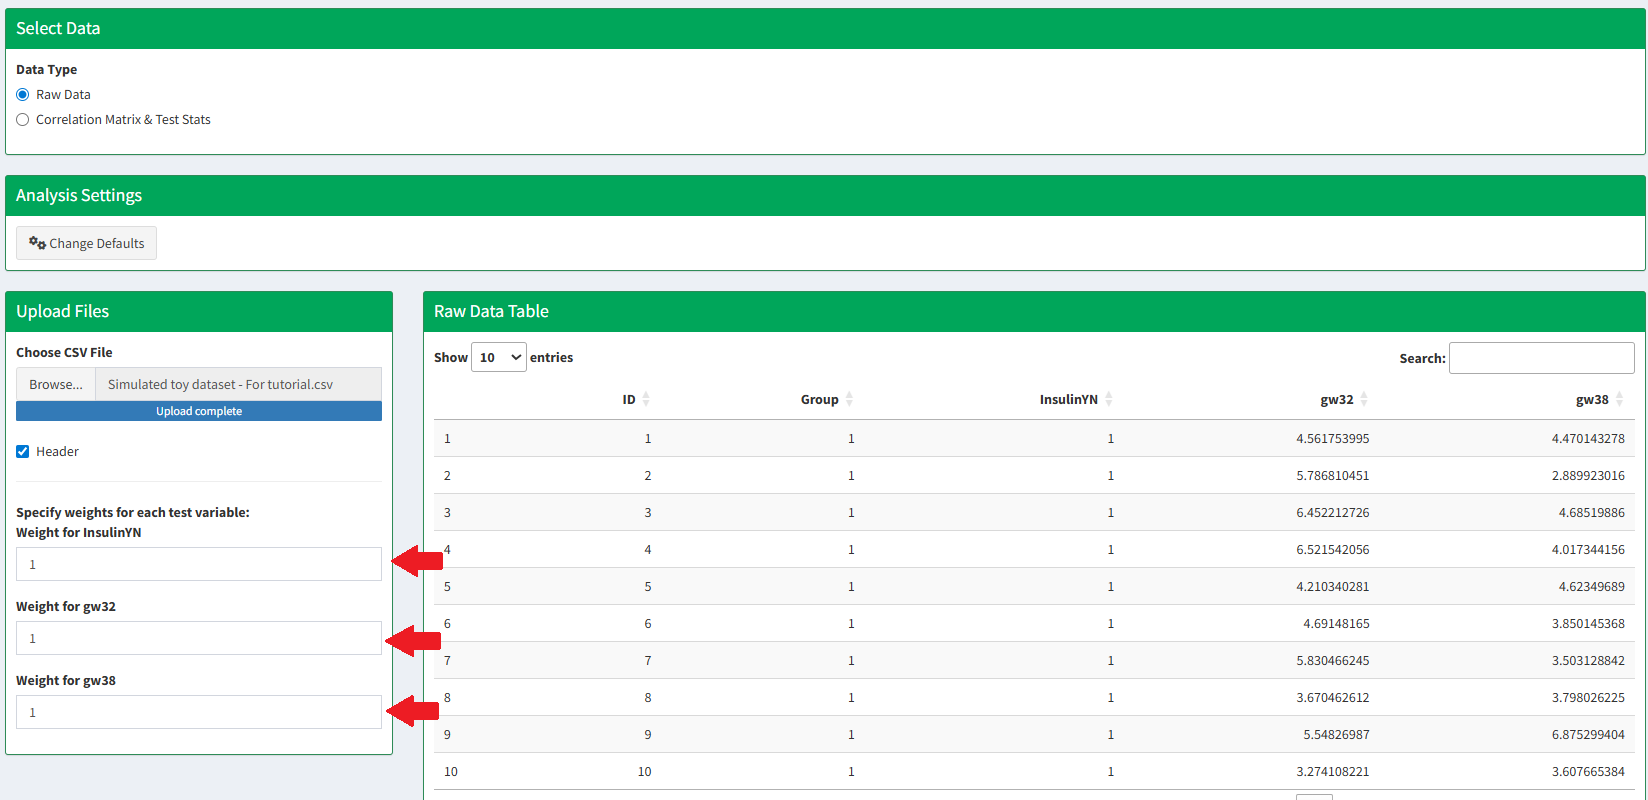
\includegraphics[width=22.89in]{SC-QC_Tutorial_Raw_Data_selection} \end{center}

The ``Analysis-QC Composite'' tab will differ slightly here, in that you
will also have to indicate which variables are categorical or survival
analysis. Once a valid raw data csv file has been uploaded, you will see
something similar to below:

\begin{center}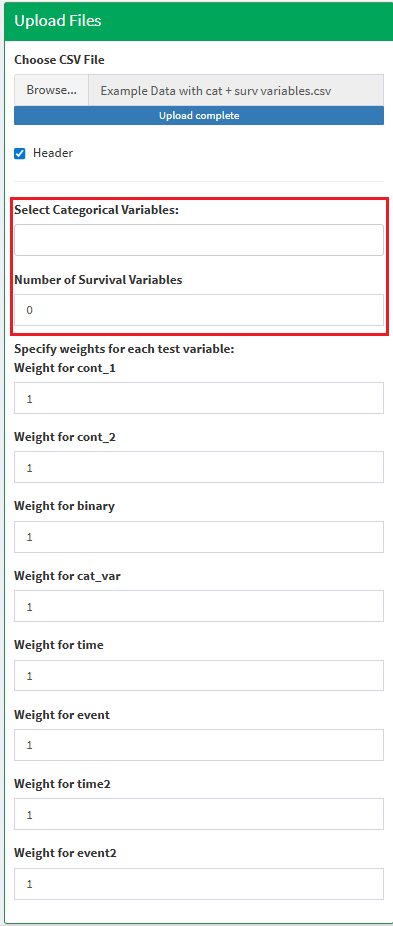
\includegraphics[width=5.46in]{QC Tutorial variable selection} \end{center}

The ``Select Categorical Variables'' box will show a drop down of all
variables in the file. Simply click on that variable to indicate that it
is categorical. Below that is a box for the number of survival analyses.
A box will be generated for each survival analysis, where you must
select the time and censor variable for that survival analysis.
\textbf{It is important to note here that the censor variable has been
encoded such that 1= censored, 0 = event}. See below an example of this
will appear.

\begin{center}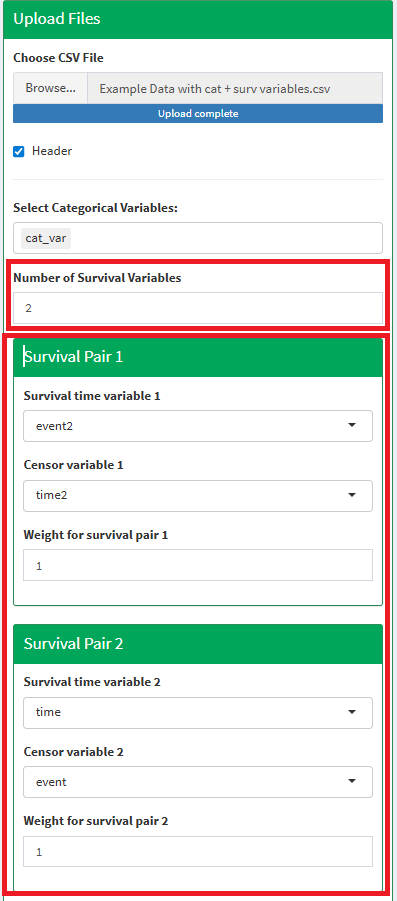
\includegraphics[width=5.51in]{Survival pair} \end{center}

\textbf{Notes on Uploading Correlation Matrix} For uploading the
correlation matrix csv, ensure that you upload only the correlation
matrix of the outcome variables of interest. Ensure that both row names
and column names are included, as seen in the example format below. The
individual test statistics must be calculated and uploaded manually by
the user.

\begin{center}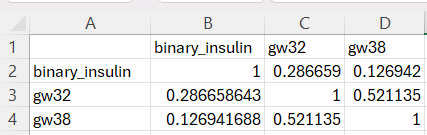
\includegraphics[width=5.93in]{Example Correlation Matrix} \end{center}

The test statistic of each variable needs to be entered into the
corresponding box for the outcome, which are displayed automatically
after a valid correlation matrix has been uploaded. Weighting for each
variable can also be applied here. Equal weighting is applied by default
(where weights are equal to 1 for all outcomes).

\begin{center}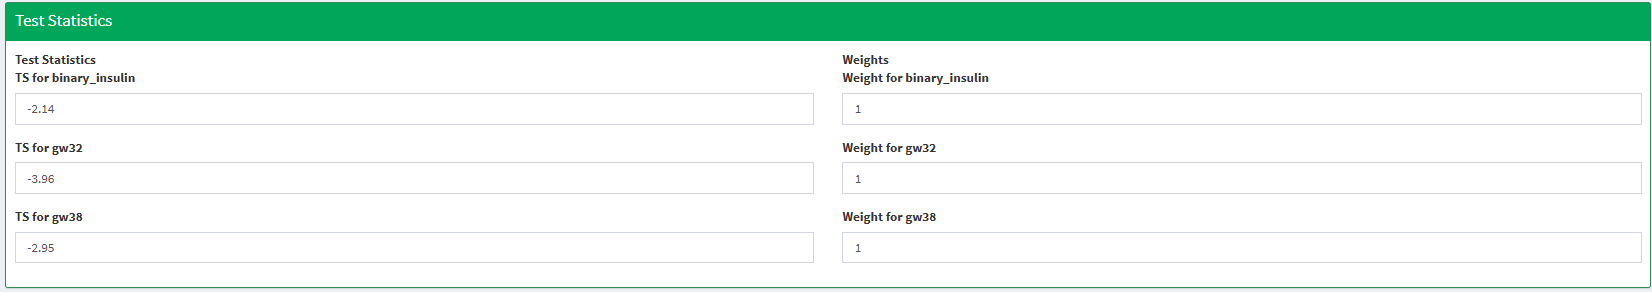
\includegraphics[width=22.74in]{SC-QC Tutorial CMTS Weights and TS} \end{center}

\textbf{General Settings} The analysis settings tab allows the user to
change some of the default settings of the analysis, including the level
of significance (\(\alpha\)), the seed used for the
simulations/permutations, and the sided-ness of the hypothesis test
(relevant only for the summed composite(SC)). These settings can be
accessed via the ``Change Defaults'' button in the Analysis Settings
box, shown below.

\begin{center}\includegraphics[width=23.21in]{Analysis Settings } \end{center}

\textbf{Notes on the Number of Permutations/Simulations} When choosing
the number of permutations/simulations to run there are two things you
must take into consideration; the complexity of the data and the
precision of the p-value. Increasing the number of
permutations/simulations will improve the precision of the reported
p-value, however this comes at increasing computational effort. Large
datasets will also increase computational costs, making large numbers of
permutations prohibitive. Generally, 500-1000 permutations/simulations
is considered acceptable, although this depends on the level of
significance. Additionally, simulating via asymptotic theory is much
more efficient than permutation testing, and can therefore handle a
larger number of simulations versus what permutation testing can handle.
Trial and error may be required to determine how many permutations can
be performed to obtain the most precise p-value possible.

\end{document}
